\chapter{Six degree-of-freedom vehicle model}
\label{chap:6dof}
\section{6DoF Model structure}
\label{sec:6dofconcept}
The state of the car is identified by the six degrees of freedom required to define the position and orientation of its chassis. The car interacts with the road through a simplified suspension system.
The model outputs are the vertical forces on each of the four wheels and the velocities of the respective ground contact points, which may be used to calculate friction by an external tyre model.
Inputs to the model are the longitudinal and lateral forces acting on each wheel and the steering angle. The latter effectively rotates the force vectors of the front wheels allowing direction control.
The block diagram in figure \ref{6flow} shows the intended flow of information for this model working in conjuction with a tyre model.
\begin{figure}[ht]
  \centering
  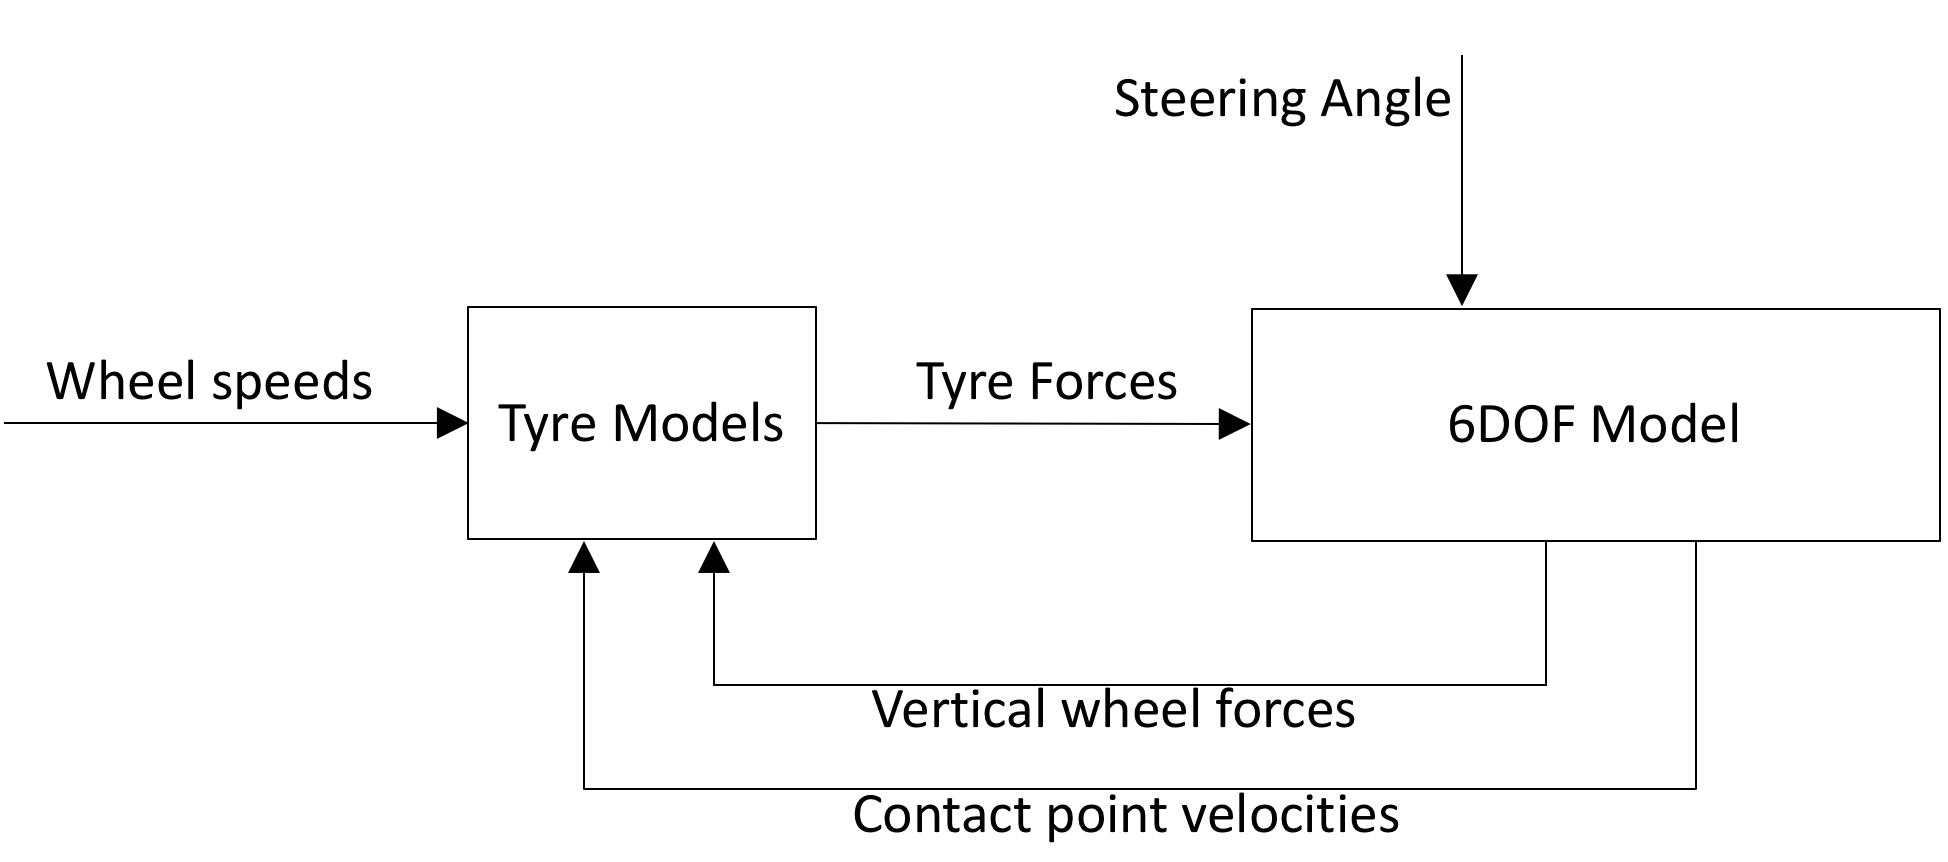
\includegraphics[width=\textwidth]{images/6flow.png}
  \caption{Information flow between the tyre model and the 6dof vehicle model.}
  \label{6flow}
\end{figure}
\section{Chassis description}
\label{sec:body}
The road is assumed to be a horizontal plane. In the $xyz$ inertial reference system $z$ is pointed downwards, in the direction of gravity whilst $x$ and $y$ lye on the road surface and may be arbitrarily chosen as long as the right-handedness of the reference frame is guaranteed.

The chassis is represented by a rigid body whose mass $m$ and rotational inertia matrix $I$ resemble those of the entire vehicle, inclusive of the driver and the wheels.

The body reference system $x'y'z'$ is fixed to the chassis and originates at the Center of Gravity. An unambiguous definition of the axes is made in the static equilibrium orientation when the suspension system is bearing the weight of the car and no other forces are at play (this will be later referenced as the \textit{resting condition}). In this condition $z'$ is defined to be parallel to $z$ and likewise pointed downwards, $x'$ is directed forwards, parallel to the road plane, and the $y'$ axis is oriented to the right of the car as seen by the driver. The chassis reference system here defined is in line with the SAE J670 definition depicted in figure \ref{saeaxes}.
\begin{figure}[ht]
  \centering
  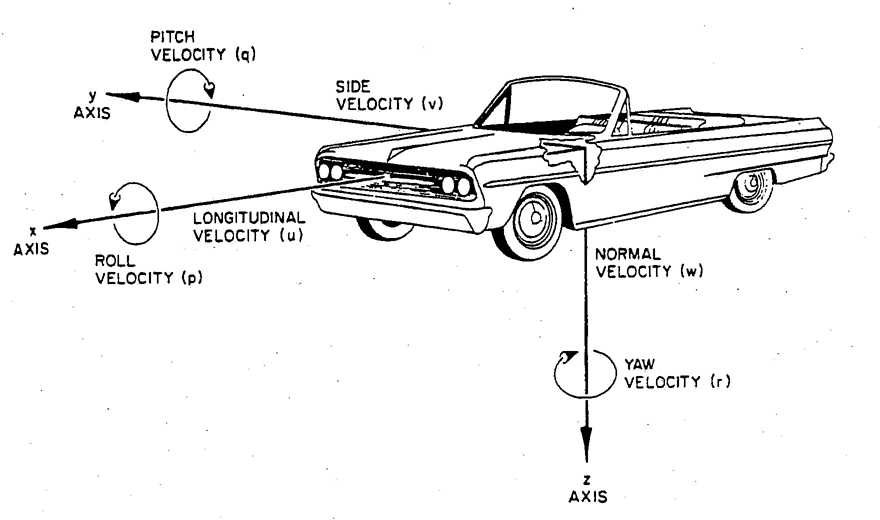
\includegraphics[height = 7cm]{images/saeaxes}
  \caption{The chassis reference system as defined in the SAE J670 standard.}
  \label{saeaxes}
\end{figure}

The attitude of the chassis is defined by the Tait-Bryan angles mapping the inertial system axes to the chassis axes \todo{appendix}. Note that the given definition for the chassis reference system implies zero roll and pitch at static equilibrium.

The chassis is assumed to be symmetrical about the $x'z'$ plane, this identifies the $y'$ axis as a principle axis of inertia and eliminates all the related product of inertia terms from the inertia matrix evaluated in the chassis reference system.
$$
I = \begin{bmatrix}
I_{xx} & 0      & I_{xz}\\
0      & I_{yy} & 0     \\
I_{xz} & 0      & I_{zz}
\end{bmatrix}.
$$

\section{Suspension}
\label{sec:suspension}
Suspension is represented by four vertical linear spring-damper systems associated with each wheel of the car. Quantities relating to each of the systems will be distinguished by subscripts according to Table \ref{table:subscripts}, the $w$ subscript is used when referring generically to any one of them.

\begin{table}[ht]
  \caption{Wheel and suspension systems subscripts} % title of Table
  \centering % used for centering table
  \begin{tabular}{l l l l} % left aligned columns (4 columns)
    \hline\hline %inserts double horizontal lines
    Subscript & Pertaining wheel or suspension system \\ [0.5ex] % inserts table
    %heading
    \hline % inserts single horizontal line
    $FR$ & Front Right \\ % inserting body of the table
    $FL$ & Front Left \\
    $RR$ & Rear Right \\
    $RL$ & Rear Left \\ [1ex] % [1ex] adds vertical space
    \hline %inserts single line
  \end{tabular}
  \label{table:subscripts} % is used to refer this table in the text
\end{table}

The upper end of each suspension system is attached to an appropriate point $P_w$ statically defined with respect to the chassis, the lower end point is obtained by projecting $P_w$ onto the road plane.
The spring length $h_w$ is given by the distance between $P_w$ and the road plane, so it is equal to the opposite of the inertial system $z$ coordinate of $P_w$.

\begin{figure}[ht]
  \centering
  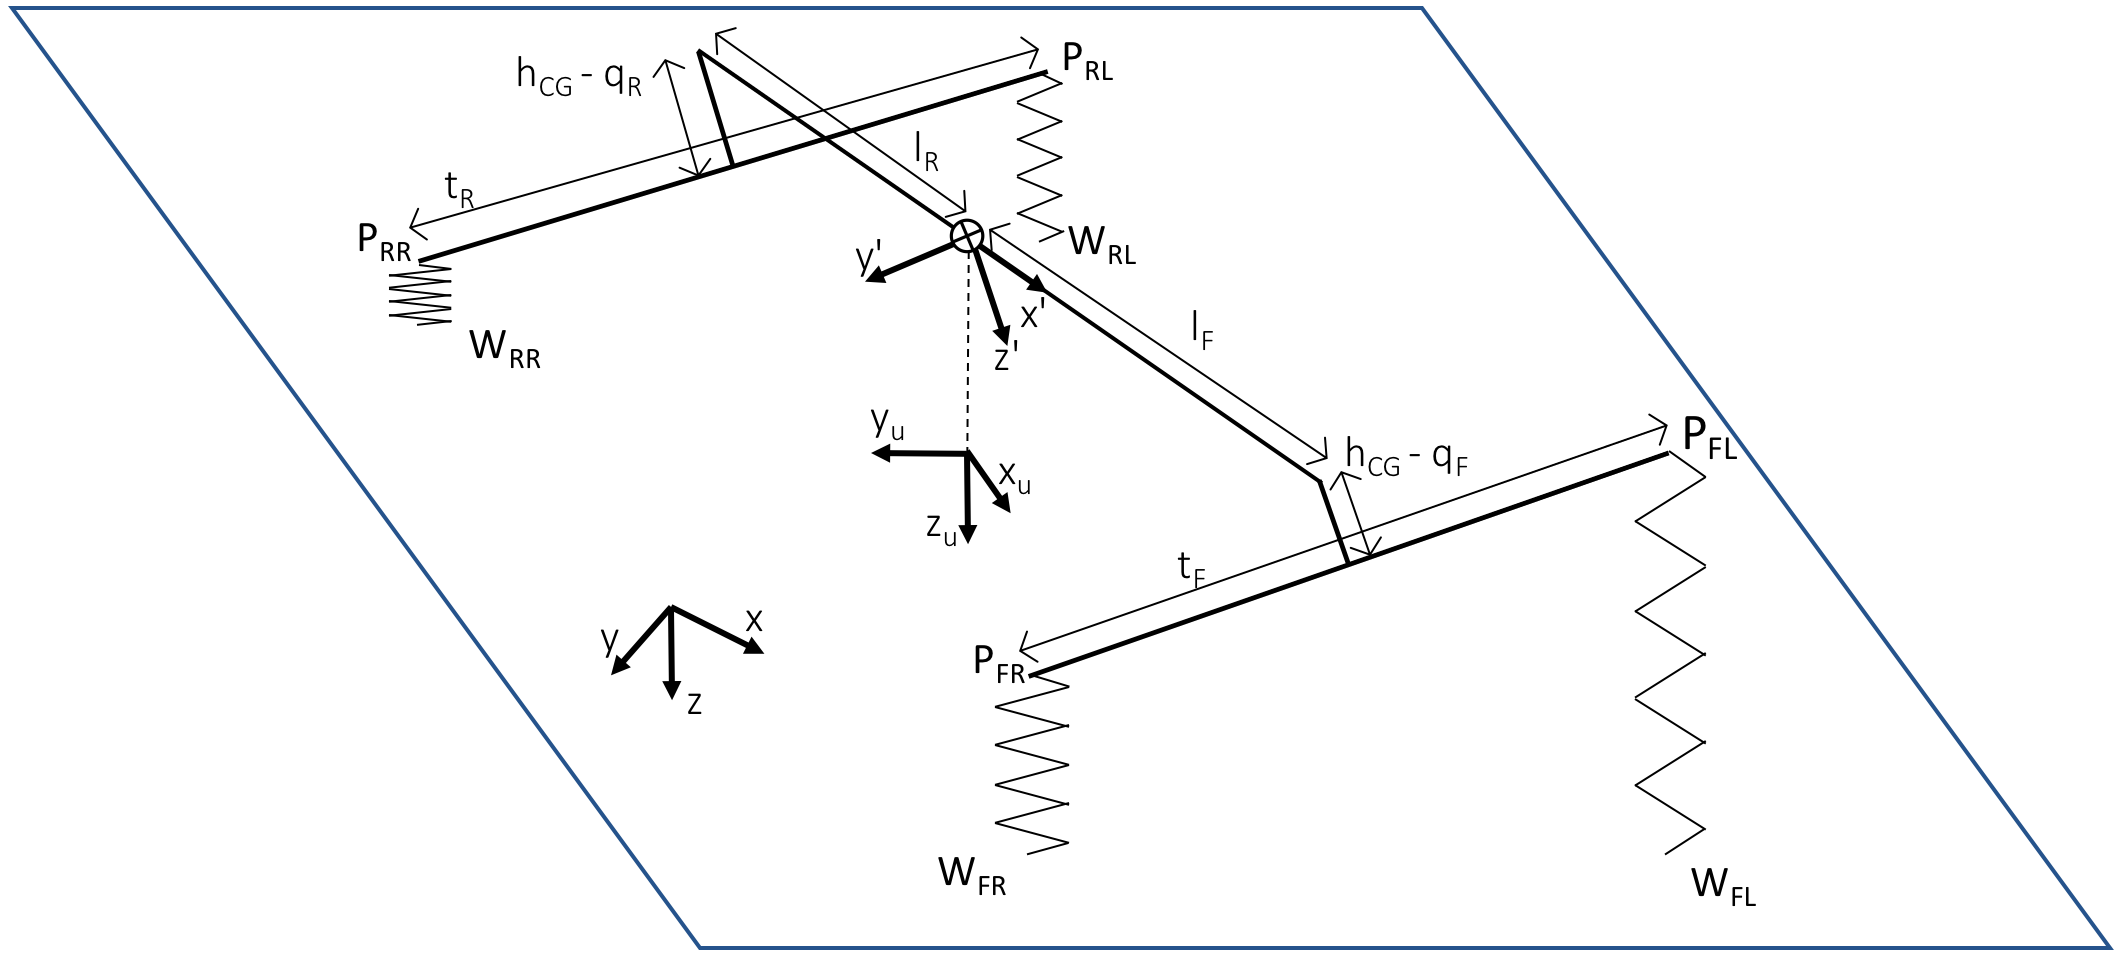
\includegraphics[width=\textwidth]{images/3dview}
  \caption{Description of the 6 DoF model geometry.}
  \label{3dview}
\end{figure}

The correct weight transfer effects are obtained by assigning the corresponding wheel contact point $x$ and $y$ coordinates to each of the $P_w$ points, these are easily calculated from the front and rear track lengths ($t_F$ and $t_R$) and the distances of the front and rear axles from the CoG ($l_F$ and $l_R$).

The $z$ co-ordinates of the $P_w$ points with respect to the chassis system are finally chosen in order to obtain realistic roll dynamics.

Automotive suspension systems can be characterized by a roll center for each axle. This is the point at which lateral forces acting on the wheels are reacted to the chassis.
The roll center is usually below the center of mass, causing vehicles to lean towards the outside of turns when driving, this is in line with the situation shown in figure \ref{roll}, where the lateral force at the center of mass is the centrifugal force acting in the non inertial reference frame of the car, balanced by friction acting on the wheel contact points.

\begin{figure}[ht]
  \centering
  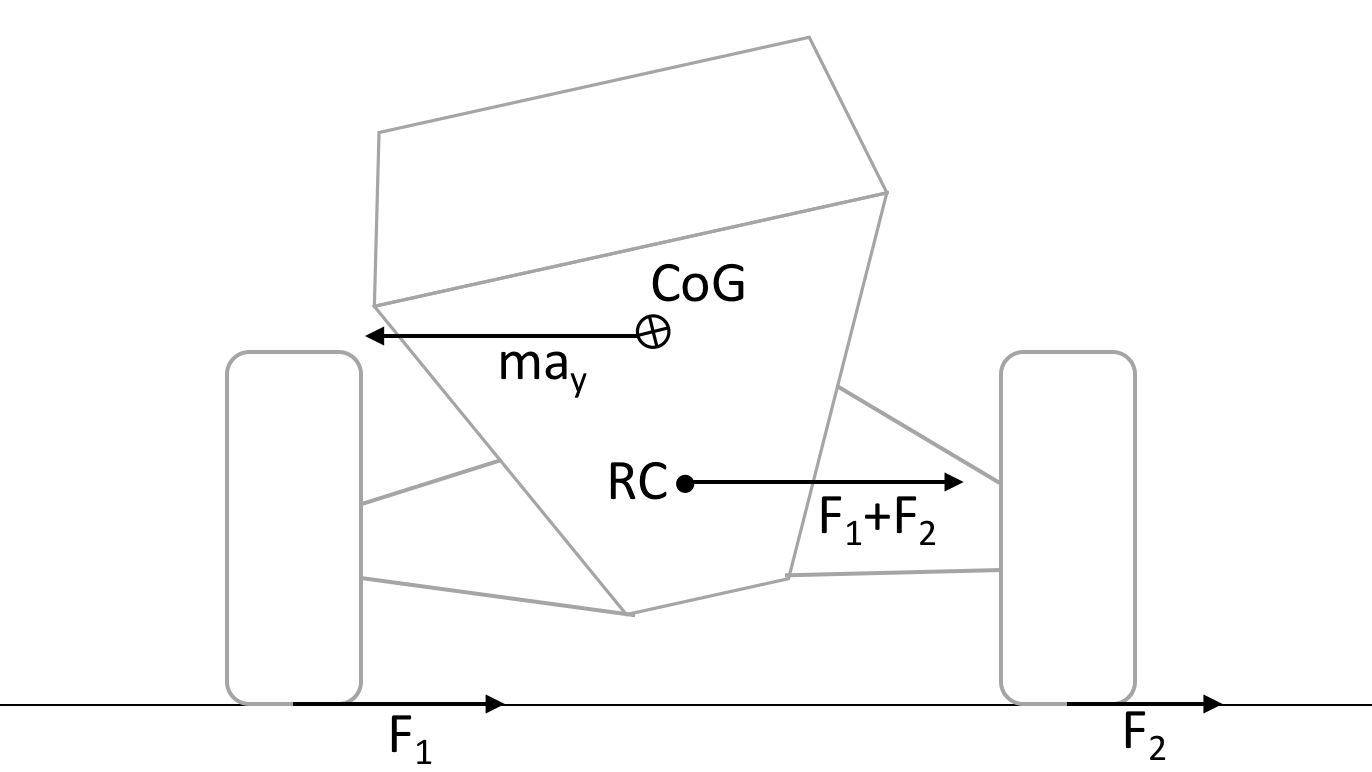
\includegraphics[height = 7cm]{images/roll}
  \caption{Body roll during cornering.}
  \label{roll}
\end{figure}

The roll center height, as defined by the SAE in J670, is determined by suspension kinematics and dynamic load distribution so it is almost never constant.
In the developed model, each roll center is approximated by the midpoint of the left and right $P_w$ points of the corresponding axle. Appendix \ref{chap:roll} justifies this approximation.

The roll center heights ($q_F$ and $q_R$) are a common design specification in race cars.
Their values can be obtained by means of multibody simulation, experimental tests or kinematic approximations.
$q_F$ and $q_R$  are given with respect to ground in the resting condition even though they are relevant when considered in respect to the CoG height and tend to move with the chassis of the vehicle.
When the model is in the resting condition the height of each of the $P_w$ points is made to match the corresponding roll center height by completing their definition as in table \ref{table:susppoints}.

\begin{table}[ht]
  \caption{Coordinates of the suspension force application points} % title of Table
  \centering % used for centering table
  \begin{tabular}{l l l l l} % left aligned columns (4 columns)
    \hline\hline %inserts double horizontal lines
    Chassis system co-ordinate & $P_{FR}$ & $P_{FL}$ & $P_{RR}$ & $P_{RL}$ \\ [0.5ex] % inserts table
    %heading
    \hline % inserts single horizontal line
    $ x$ & $ l_f$ & $ l_f$ & $-l_r $ & $-l_r $\\ % inserting body of the table
    $ y$ & $ \frac{t_f}{2} $ & $ -\frac{t_f}{2}$ & $ \frac{t_r}{2}$ & $ -\frac{t_r}{2}$\\ % inserting body of the table
    $ z$ & $ h_{CG} - q_F $& $ h_{CG} - q_F $ & $ h_{CG} - q_R$ & $ h_{CG} - q_R$ \\ [1ex] % [1ex] adds vertical space
    \hline %inserts single line
  \end{tabular}
  \label{table:susppoints} % is used to refer this table in the text
\end{table}

Appendix \ref{chap:roll} also shows that the linear spring rates for the model should be chosen as
$$
k_F = \frac{\phi}{F} = 2\frac{h_{CG}-q_F}{K_{\phi F} t_F^2}.
$$
$$
k_R = \frac{\phi}{F} = 2\frac{h_{CG}-q_R}{K_{\phi R} t_F^2}.
$$

To make the model of the car sit in the resting position with zero pitch angle and the correct CoG height the unloaded spring lengths must be
$$ h_{F0} = q_F + \frac{mg}{2k_F}\frac{l_R}{l_R+l_F} $$
$$ h_{R0} = q_r + \frac{mg}{2k_R}\frac{l_F}{l_R+l_F} $$

\section{Lagrangian formulation of the problem}
\label{sec:6doflag}
Equations of motion were obtained by solving the lagrangian formulation of the system with respect to the inertial reference frame.
The chosen lagrangian coordinates are, in order, the yaw, pitch and roll angles and the coordinates of the chassis CoG
$$
q = \begin{bmatrix}
\psi \\
\theta \\
\phi \\
x_{CG} \\
y_{CG} \\
z_{CG}
\end{bmatrix}.
$$
The gravitational potential energy is
$$U_{grav} = -mgz_{CG}$$
The potential energy stored in the suspension springs is
$$ U_{spring} = \frac{1}{2} k_F [(h_{FR} - h_{F0})^2 + (h_{FL} - h_{F0})^2] +  \frac{1}{2} k_R [(h_{RR} - h_{R0})^2 + (h_{RL} - h_{R0})^2] $$

The total potential energy function is
$$ U = U_{spring} + U_{grav} $$

The damping effect of the suspension is modelled by the Rayleigh dissipation function
$$ D = \frac{1}{2} b_F (\dot h_{FR}^2 + \dot h_{FL}^2) + \frac{1}{2} b_R (\dot h_{RR}^2 + \dot h_{RL}^2) $$
$b_F$ and $b_r$ are the damping ratios of the spring damper systems. \todo{how to get these parameters?}

The translational kinetic energy of the car is given by
$$ T_{trans} = \frac{1}{2} m (\dot x_{CG}^2 +\dot y_{CG}^2 +\dot z_{CG}^2 ) $$

The rotational kinetic energy is obtained from the expression
$$ T_{rot} = \frac{1}{2}\omega^T I \omega $$

The angular velocity vector $\omega$ must be expressed with respect to the same axes as the inertia matrix, i.e. the chassis reference frame.

The total kinetic energy function is then
$$ T = T_{rot} + T_{trans} $$

The steering angle input $\delta$ acts like a time varying parameter in the model, influencing the wheel system rotation matrices.
The tyre horizontal force component inputs $F_wx$ $F_wy$ are to be expressed with respect to each of the wheel reference systems.

To obtain the generalized forces vector $Q$. The external forces are rotated into inertial frame co-ordinates and applied to the $W_w$ points.

\section{6DoF Dynamics equation set}
\label{sec:6dofeq}
\todo{districare il groviglio che mi lascia Matlab}

\section{Output functions}
\label{sec:6dofout}
The vertical wheel load outputs are calculated by the forces acting in the suspension systems, as a sum of the elastic and linear damping force.
$$Z_{FR} = - k_F (h_{FR} - h_{F0}) - b_F \dot h_{FR} $$
$$Z_{FL} = - k_F (h_{FL} - h_{F0}) - b_F \dot h_{FL} $$
$$Z_{RR} = - k_R (h_{RR} - h_{R0}) - b_R \dot h_{RR} $$
$$Z_{RL} = - k_R (h_{RL} - h_{R0}) - b_R \dot h_{RL} $$

The contact point velocities output is given by the time derivatives of the $W_w$ points' co-ordinates in the inertial frame rotated into wheel system co-ordinates. The $W_w$ point coordinates are defined with respect to the undercarriage reference frame in table \ref{table:contactpoints}

\begin{table}[ht]
  \caption{Coordinates of the tyre contact points} % title of Table
  \centering % used for centering table
  \begin{tabular}{l l l l l} % left aligned columns (4 columns)
    \hline\hline %inserts double horizontal lines
    Undercarriage system co-ordinates & $W_{FR}$ & $W_{FL}$ & $W_{RR}$ & $W_{RL}$ \\ [0.5ex] % inserts table
    %heading
    \hline % inserts single horizontal line
    $ x$ & $ l_f$ & $ l_f$ & $-l_r $ & $-l_r $\\ % inserting body of the table
    $ y$ & $ \frac{t_f}{2} $ & $ -\frac{t_f}{2}$ & $ \frac{t_r}{2}$ & $ -\frac{t_r}{2}$\\ % inserting body of the table
    $ z$ & $ 0 $& $ 0 $ & $ 0$ & $ 0$ \\ [1ex] % [1ex] adds vertical space
    \hline %inserts single line
  \end{tabular}
  \label{table:contactpoints} % is used to refer this table in the text
\end{table}

The outputs expressed as fuctions of the lagrangian coordinates are:
\todo{districa matlab}
The Lagrange Equations may be expressed in the form

$$M(\theta,\phi)\ddot x = f(q, \dot q) + Q(\delta)u$$

\begin{align*}
  M_{\mathrm{\psi},\mathrm{\psi}}&=\mathrm{I_{zz}}\,{\cos\left(\mathrm{\theta}\right)}^2\,{\cos\left(\mathrm{\phi}\right)}^2+\mathrm{I_{yy}}\,{\cos\left(\mathrm{\theta}\right)}^2\,{\sin\left(\mathrm{\phi}\right)}^2-2\,\mathrm{I_{xz}}\,\cos\left(\mathrm{\theta}\right)\,\cos\left(\mathrm{\phi}\right)\,\sin\left(\mathrm{\theta}\right)+\mathrm{I_{xx}}\,{\sin\left(\mathrm{\theta}\right)}^2 \\
  M_{\mathrm{\psi},\mathrm{\theta}}&=\sin\left(\mathrm{\phi}\right)\,\left(\mathrm{I_{xz}}\,\sin\left(\mathrm{\theta}\right)+\mathrm{I_{yy}}\,\cos\left(\mathrm{\theta}\right)\,\cos\left(\mathrm{\phi}\right)-\mathrm{I_{zz}}\,\cos\left(\mathrm{\theta}\right)\,\cos\left(\mathrm{\phi}\right)\right) \\
  M_{\mathrm{\psi},\mathrm{\phi}}&=\mathrm{I_{xz}}\,\cos\left(\mathrm{\theta}\right)\,\cos\left(\mathrm{\phi}\right)-\mathrm{I_{xx}}\,\sin\left(\mathrm{\theta}\right) \\
  M_{\mathrm{\theta},\mathrm{\theta}}&=\mathrm{I_{yy}}-\mathrm{I_{yy}}\,{\sin\left(\mathrm{\phi}\right)}^2+\mathrm{I_{zz}}\,{\sin\left(\mathrm{\phi}\right)}^2 \\
  M_{\mathrm{\theta},\mathrm{\phi}}&=-\mathrm{I_{xz}}\,\sin\left(\mathrm{\phi}\right) \\
  M_{\mathrm{\phi},\mathrm{\phi}}&=\mathrm{I_{xx}}
\end{align*}


$$
M(\phi,\theta)=\left(\begin{array}{cccccc} M_{\mathrm{\psi},\mathrm{\psi}} & M_{\mathrm{\psi},\mathrm{\theta}} & M_{\mathrm{\psi},\mathrm{\phi}} & 0 & 0 & 0\\ M_{\mathrm{\psi},\mathrm{\theta}} & M_{\mathrm{\theta},\mathrm{\theta}} & M_{\mathrm{\theta},\mathrm{\phi}} & 0 & 0 & 0\\ M_{\mathrm{\psi},\mathrm{\phi}} & M_{\mathrm{\theta},\mathrm{\phi}} & M_{\mathrm{\phi},\mathrm{\phi}} & 0 & 0 & 0\\ 0 & 0 & 0 & m & 0 & 0\\ 0 & 0 & 0 & 0 & m & 0\\ 0 & 0 & 0 & 0 & 0 & m \end{array}\right)
$$
